%%%%%%%%%%%%%%%%%%%%%%%%%%%%%%%%%%%%%%%%%%%%%%%%%%%%%%%%%%%%%%%%%%%%%%%%%%%%%%%%%%%%%%%%%%%%%%%%
%
% CS484 Written Question Template
%
% Acknowledgements:
% The original code is written by Prof. James Tompkin (james_tompkin@brown.edu).
% The second version is revised by Prof. Min H. Kim (minhkim@kaist.ac.kr).
%
% This is a LaTeX document. LaTeX is a markup language for producing 
% documents. Your task is to fill out this document, then to compile 
% it into a PDF document. 
%
% 
% TO COMPILE:
% > pdflatex thisfile.tex
%
% If you do not have LaTeX and need a LaTeX distribution:
% - Personal laptops (all common OS): www.latex-project.org/get/
% - We recommend latex compiler miktex (https://miktex.org/) for windows,
%   macTex (http://www.tug.org/mactex/) for macOS users.
%   And TeXstudio(http://www.texstudio.org/) for latex editor.
%   You should install both compiler and editor for editing latex.
%   The another option is Overleaf (https://www.overleaf.com/) which is 
%   an online latex editor.
%
% If you need help with LaTeX, please come to office hours. 
% Or, there is plenty of help online:
% https://en.wikibooks.org/wiki/LaTeX
%
% Good luck!
% Min and the CS484 staff
%
%%%%%%%%%%%%%%%%%%%%%%%%%%%%%%%%%%%%%%%%%%%%%%%%%%%%%%%%%%%%%%%%%%%%%%%%%%%%%%%%%%%%%%%%%%%%%%%%
%
% How to include two graphics on the same line:
% 
% \includegraphics[\width=0.49\linewidth]{yourgraphic1.png}
% \includegraphics[\width=0.49\linewidth]{yourgraphic2.png}
%
% How to include equations:
%
% \begin{equation}
% y = mx+c
% \end{equation}
% 
%%%%%%%%%%%%%%%%%%%%%%%%%%%%%%%%%%%%%%%%%%%%%%%%%%%%%%%%%%%%%%%%%%%%%%%%%%%%%%%%%%%%%%%%%%%%%%%%

\documentclass[11pt]{article}

\usepackage[english]{babel}
\usepackage[utf8]{inputenc}
\usepackage[colorlinks = true,
            linkcolor = blue,
            urlcolor  = blue]{hyperref}
\usepackage[a4paper,margin=1.5in]{geometry}
\usepackage{stackengine,graphicx}
\usepackage{fancyhdr}
\setlength{\headheight}{15pt}
\usepackage{microtype}
\usepackage{times}
\usepackage{booktabs}
\usepackage{listings}
\usepackage{xcolor}
\usepackage{amsmath}
\lstdefinestyle{codestyle}{
	frame=single,
	basicstyle=\ttfamily\footnotesize,
	keywordstyle=\bfseries\color{magenta},
	commentstyle=\itshape\color{gray},
	stringstyle=\color{orange},
	numberstyle=\sffamily\scriptsize\color{gray},
	showspaces=false,
	showstringspaces=false,
	showtabs=false,
	tabsize=4,
	breakatwhitespace=false,
	breaklines=true,
	keepspaces=true,
	captionpos=b,
	numbers=left,
	numbersep=5pt}
\lstset{style=codestyle}

\frenchspacing
\setlength{\parindent}{0cm} % Default is 15pt.
\setlength{\parskip}{0.3cm plus1mm minus1mm}

\pagestyle{fancy}
\fancyhf{}
\lhead{Homework Writeup}
\rhead{CS484}
\rfoot{\thepage}

\date{}

\title{\vspace{-1cm}Homework 3 Writeup}


\begin{document}
\maketitle
\vspace{-3cm}
\thispagestyle{fancy}

\section*{Instructions}
\begin{itemize}
  \item Describe any interesting decisions you made to write your algorithm.
  \item Show and discuss the results of your algorithm.
  \item Feel free to include code snippets, images, and equations.
  \item \textbf{Please make this document anonymous.}
\end{itemize}

\section*{Bayer Image Interpolation}

First part of this project is to make the code that interpolating the given bayer image into proper RGB image. 

\begin{lstlisting}[language=python]
def bayer_to_rgb_bilinear(bayer_img):
    
    height, width = bayer_img.shape
    rgb_img = np.zeros((height + 2, width + 2, 3), dtype=np.uint8)
    # added zero padding of 1 pixel width around the image for calculation efficiency    
    # Extract bayer image into each channel of rgb image
    # Range starts from 1 due to the padding
    rgb_img[1:-1:2, 1:-1:2, 0] = bayer_img[0::2, 0::2]    
    rgb_img[1:-1:2, 2:-1:2, 1] = bayer_img[0::2, 1::2]
    rgb_img[2:-1:2, 1:-1:2, 1] = bayer_img[1::2, 0::2]
    rgb_img[2:-1:2, 2:-1:2, 2] = bayer_img[1::2, 1::2]

    # For the R channel
    rgb_img[1:height:2, 2:width+1:2, 0] = (rgb_img[1:height:2, 1:width:2,0]//2 + 
    rgb_img[1:height:2, 3:width+2:2,0]//2) 
    rgb_img[2:height+1:2, 1:width:2, 0] = (rgb_img[1:height:2, 1:width:2,0]//2 + 
    rgb_img[3:height+2:2, 1:width:2,0]//2) 

    rgb_img[2:height+1:2, 2:width+1:2, 0] = (
        rgb_img[1:height:2, 1:width:2, 0]//4 + 
        rgb_img[1:height:2, 3:width+2:2, 0]//4 +
        rgb_img[3:height+2:2, 1:width:2, 0]//4 + 
        rgb_img[3:height+2:2, 3:width+2:2, 0]//4
    ) 
    #For the G channel
    rgb_img[1:-1:2, 1:-1:2, 1] = (
        rgb_img[1:-1:2, 0:-2:2, 1]//4 + 
        rgb_img[0:-2:2, 1:-1:2, 1]//4 +
        rgb_img[2::2, 1:-1:2, 1]//4 + 
        rgb_img[1:-1:2, 2::2, 1]//4
    )
    rgb_img[2:height+1:2, 2:width+1:2, 1] = (
        rgb_img[2:height+1:2, 1:width:2, 1]//4 + 
        rgb_img[1:height:2, 2:width+1:2, 1]//4 +
        rgb_img[3:height+2:2, 2:width+1:2, 1]//4 + 
        rgb_img[2:height+1:2, 3:width+2:2, 1]//4
    )

    # For the B channel
    rgb_img[2::2, 1:-2:2, 2] = (rgb_img[2::2, 0:-3:2,2]//2 +
    rgb_img[2::2, 2:-1:2,2]//2) 
    rgb_img[1:-2:2, 2::2, 2] = (rgb_img[0:-3:2, 2::2,2]//2 +
    rgb_img[2:-1:2, 2::2,2]//2) 
    
    rgb_img[1:-2:2, 1:-2:2, 2] = (
        rgb_img[0:-3:2, 0:-3:2, 2]//4 + 
        rgb_img[0:-3:2, 2:-1:2, 2]//4 +
        rgb_img[2:-1:2, 0:-3:2, 2]//4 + 
        rgb_img[2:-1:2, 2:-1:2, 2]//4
    )    
    #Remove Padding
    rgb_img = rgb_img[1:-1, 1:-1, :]
    
    return rgb_img
    \end{lstlisting}

I'll explain my code step by step. 


\begin{enumerate}
    \item First, I made the empty array for result image with 2 pixels bigger than bayer image. This is because I wanted to add zero padding of 1 pixel around the image, for edge calculation.
    \item Then I brought the each R,G,B pixels from the bayer image and applied to channels in R,G,B order. To apply padding, i left the first and last pixels zero and filled the pixel value starting from 1.
    \item For each channel, used bilinear interpolation to fill the missing pixel values. I used indexing and slicing of Numpy to do this, since it is much faster than naive for loops. I first diveded the value and then sum up, because when I summed up first it overflowed the index RGB value (from 0 to 255), so to avoid this I devided first.
    \item For the pixels in edges, I just used the same ways with other pixels, the only difference is that averaged the zero padding together. This makes the edge value smaller than intended, but it could the code more precise.
    \item Finally, I removed the zero padding by slicing the result image from the first pixel to the second last pixel.
\end{enumerate}

These are two images obatained from bilinear interpolation.

\begin{figure}
    \centering
    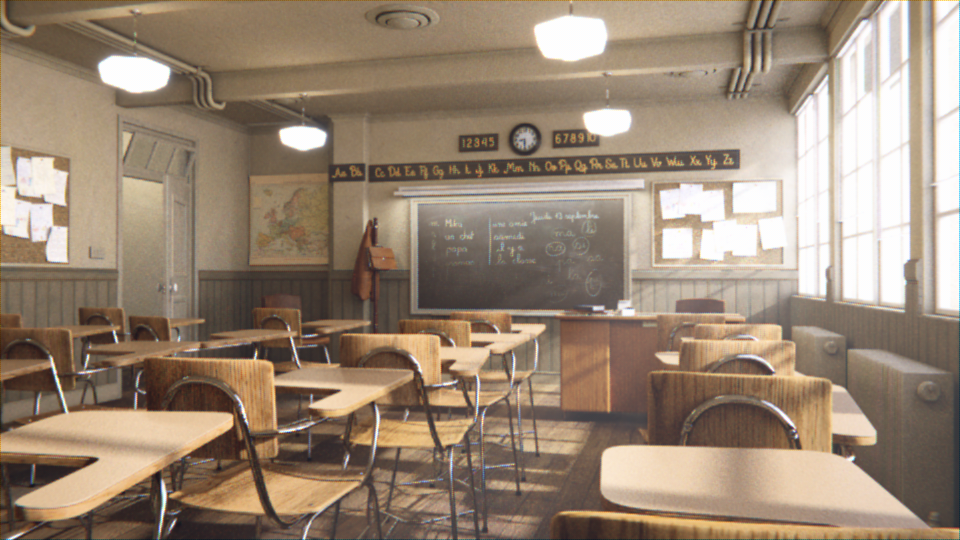
\includegraphics[width=5.5cm]{../result/bilinear_img1.png}
    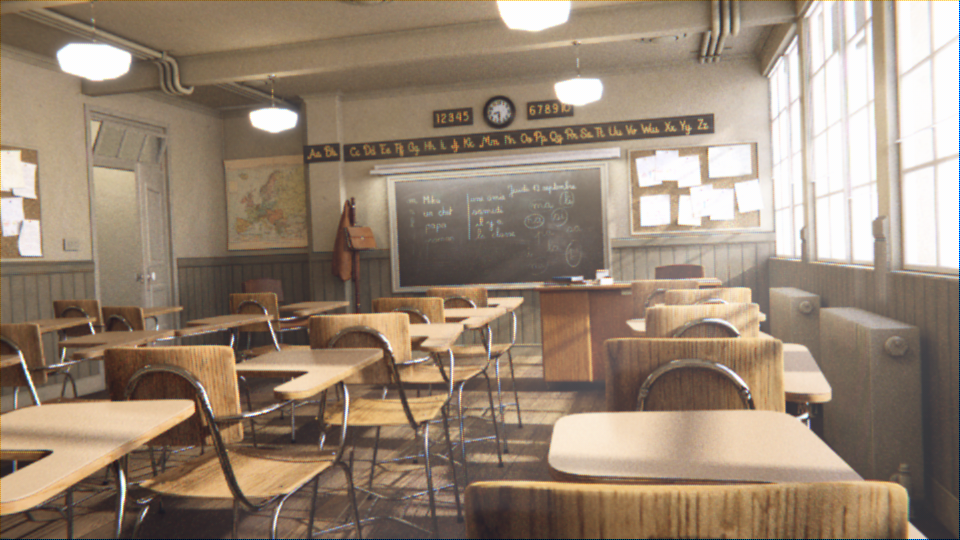
\includegraphics[width=5.5cm]{../result/bilinear_img2.png}
\caption{Images obtained from bilienear interpolation}
\end{figure}

The problem in this implementation is as mentioned, the edge control. I think this could be resolved by using other methods for edges, such as reflection.


\section*{Fundamental Matrix Calculation}
In this section, with given 8 points on both images I obtained the fundamental matrix, using eight-point algorithm.

\begin{lstlisting}[language=python]
def calculate_fundamental_matrix(pts1, pts2):
    assert pts1.shape[1] == 2 and pts2.shape[1] == 2
    assert pts1.shape[0] == pts2.shape[0]
    
    n = pts1.shape[0]
    
    
    pts1_normalized, T1 = normalize_points(pts1.T, 2)
    pts2_normalized, T2 = normalize_points(pts2.T, 2)
    
    # Transpose back to original structure
    pts1_normalized = pts1_normalized.T
    pts2_normalized = pts2_normalized.T
    
    A = np.zeros((n, 9))
    for i in range(n):
        x1, y1 = pts1_normalized[i]
        x2, y2 = pts2_normalized[i]
        A[i] = [x1*x2, x2*y1, x2, y2*x1, y1*y2, y2, x1, y1, 1]
    
    U, S, Vt = np.linalg.svd(A)
    f = Vt[-1]
    F = f.reshape(3, 3)
    
    U, S, Vt = np.linalg.svd(F)
    S[-1] = 0
    F = U @ np.diag(S) @ Vt
    
    # Denormalize
    F = T2.T @ F @ T1
    
    return F
\end{lstlisting}
\begin{enumerate}
    \item \textbf{Normalization}
    First, I normalized the given points using the built-in fuction $normalize\_points()$. Since the function needs input coordinates with x,y in column, I transposed the given points vector and applied the function.
    Then I transposed the result of function to obtain original structure.
    
    \item \textbf{Constructing Matrix A}
    Matrix $A$ is constructed using the normalized points. I just simply put each values in the matrix, and the values come from what we learned in class and supplementary slides.
    
    \item \textbf{Singular Value Decomposition and Reshaping f}
    Performed singular value decomposition for matrix $A$, to obtain $f$.Since $f$ corresponds to the eigenvector of $A^{T}A$ with the smallest eigenvalue, I extracted the last row of $Vt$. Then, reshaped it into 3{x}3 matrix. Matrix $F$ is 3{x}3 fundmental matrix obtained from SVD.
    
    \item \textbf{Enforce F to have Rank 2, and Recalculate F}
    Performed singular value decomposition again for matrix $F$. To enforce rank 2 condition, I set the last row of S (minimum sigular value) zero and recalculated $F$ with new S.
    
    \item \textbf{Denormalization}
    Finally, I denormalized fundamental matrix $F$ with scaling matrix $T1$ and $T2$ to bring it back to the scale of the original points.
\end{enumerate}

\section*{Stereo Rectification}
\begin{lstlisting}[language=python]
def transform_fundamental_matrix(F, h1, h2):
    
    
    F_mod = np.linalg.inv(h2).T @ F @ np.linalg.inv(h1)
    
    return F_mod

def rectify_stereo_images(img1, img2, h1, h2):
    
    height, width = img1.shape[:2]
        
    pts = np.float32([[0, 0], [width - 1, 0], [width - 1, height - 1], [0, height - 1]]).reshape(-1, 1, 2)

    dst1 = cv2.perspectiveTransform(pts, h1)
    dst2 = cv2.perspectiveTransform(pts, h2)
    # Calculate the bounding box dimensions
    x_min1, y_min1 = np.int32(dst1.min(axis=0))[0]
    x_max1, y_max1 = np.int32(dst1.max(axis=0))[0]
    x_min2, y_min2 = np.int32(dst2.min(axis=0))[0]
    x_max2, y_max2 = np.int32(dst2.max(axis=0))[0]

    x_min = min(x_min1, x_min2)
    y_min = min(y_min1, y_min2)
    x_max = max(x_max1, x_max2)
    y_max = max(y_max1, y_max2)

    T1 = np.array([[1, 0, -x_min + 50],
            [0, 1, -y_min + 50],
            [0, 0, 1]])
    T2 = np.array([[1, 0, -x_min + 50],
                [0, 1, -y_min + 50],
                [0, 0, 1]])

    h1_mod = T1 @ h1
    h2_mod = T2 @ h2

    new_size = (x_max - x_min + 100, y_max - y_min + 100)

    img1_rectified = cv2.warpPerspective(img1, h1_mod, new_size)
    img2_rectified = cv2.warpPerspective(img2, h2_mod, new_size)


    return img1_rectified, img2_rectified, h1_mod, h2_mod
\end{lstlisting}
\begin{enumerate}
    \item \textbf{transform\_fundamental\_matrix} In this, I just simply made new fundamental matrix with the given homographies, $F_{mod}=H_2^{-T}FH_1^{-1}$
    \item Next, I changed the homography matrices to avoid cropping. To implement this, I transformed the corner points first and set the edge of rectified images with the boundary. Details are explained below.
    \item \textbf{Defining Corner Points} First, I defined the corner points of the imgae in $pts$. After calculating new homography, the points are translated to new point with it to obtain the boundary of rectified image.
    
    \item \textbf{Calculate Transformed Points} The corner points are transformed using the original homography matrices $H$ and $H'$ for both images. 
    
    I used $cv2.perspectiveTransform()$ with corner points and homography matrix, to apply transform in the corner points.

    \item \textbf{Bounding Box Calculation} I obtained the coordinates of two bounding boxes from each images by choosing the minimum and maximum values among the corner point coordinates transformed by $cv2.perspectiveTransform()$. Since the result of transform is float value, I rounded them to integer by $np.int32$, and made into 1-dimensional array.
    \item Furthermore, I chose the minimum and maximum value among two boundaries of each images, to set the translation matrix with respect of bigger value. I did this because we should use box that could contain both images, thus we should use the bigger box to not crop the image.
    \item \textbf{Translation Matrices} By the coordinate of boundaries obtained in previous step, I constructed the translation matrices. I added margin of 50 pixels around the images, to make it not tightly stick to the edge and look like what in the supplementary slides.
    \item \textbf{Modified Homographies} The original homography matrices are modified using the translation matrices, and obtained two new homography matrices.
    \item \textbf{Warp Image} Finally, I applied $cv2.warpPerspective()$ to warp the images using the modified homography matrices and obtain the rectified images. Value $new\_size$ is the size of final image after warp, which contains margin of 50 pixels for four directions around the image. The result is below.
    
\end{enumerate}
\begin{figure}[h]
    \centering
    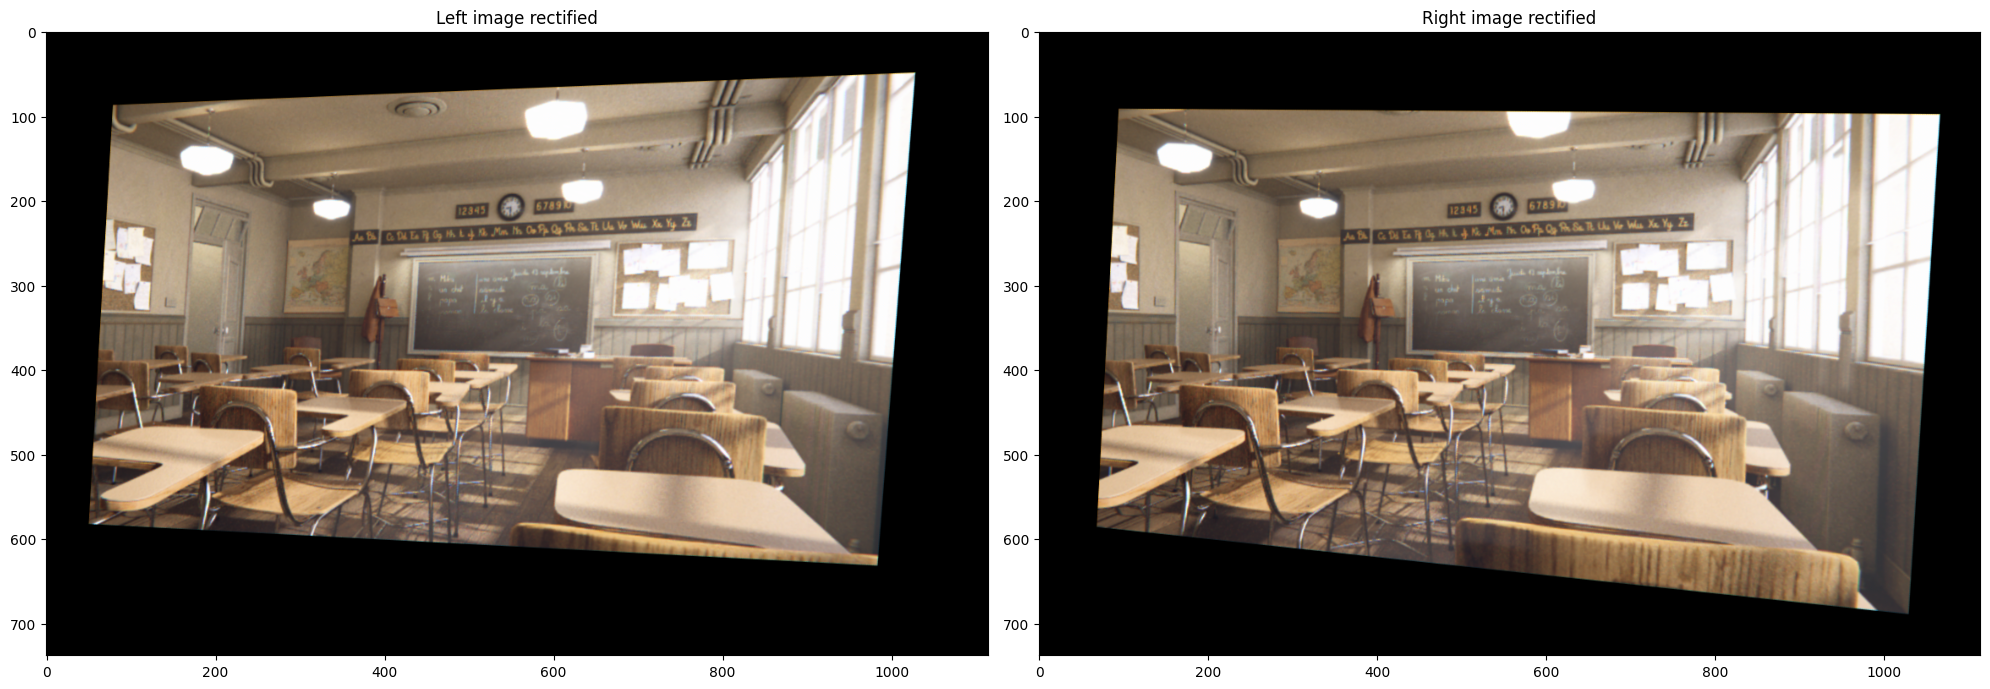
\includegraphics[width=12cm]{../result/rectified_imgs_result.png}
    \caption{Rectified Images}
    \label{fig:result1}
\end{figure}
The fundamental matrices obtained from each function is like this.
\[\left[
\begin{matrix}
    1.13843181e-21 & -3.30364530e-16 & -1.02724445e-15\\
    2.56400517e-18 & -4.61081404e-17 & 9.19265708e-01\\
    9.69843866e-17 & -9.19265708e-01 & 4.87118170e-14
\end{matrix}
\right] \]
\[\left[
\begin{matrix}
    8.24589712-22 & -3.30459784e-16 & 3.03620926e-14\\
    2.49922896e-18 & -4.61042020e-17 & 9.19265708e-01\\
    -1.37016042e-16 & -9.19265708e-01 & -3.16691741e-12\\
\end{matrix}
\right]\]
If matrix $F$ is a fundamental matrix related to two recified images, it should satisfy the constraint
\[\left[
    \begin{matrix}
        0 & 0 & 0\\
        0 & 0 & T\\
        0 & -T & 0\\
    \end{matrix}
\right]\]
If we check for the new fundamental matrix of non-cropped recified image that i implemented, seven values are almost zero, and we could find out
two values $9.19265708e-01$ and $-9.19265708e-01$ satisfies the constraint given above.

\section*{Calculating Disparity Map}
The final, and the most complex part of this project is cacluating the disparity map.
\begin{lstlisting}[language=python]
def calculate_disparity_map(img1, img2):
    
    # First convert color image to grayscale
    img1_gray = cv2.cvtColor(img1, cv2.COLOR_RGB2GRAY)
    img2_gray = cv2.cvtColor(img2, cv2.COLOR_RGB2GRAY)
    # You have to get disparity (depth) of img1 (left)
    # i.e., I1(u) = I2(u + d(u)),
    # where u is pixel positions (x,y) in each images and d is dispairty map.
    # Your code here
    
    
    h, w = img1_gray.shape
    half_window = WINDOW_SIZE // 2
    
    # Initialize disparity map and cost volume
    disparity_map = np.zeros((h, w), dtype=np.float32)
    cost_volume = np.zeros((h, w, DISPARITY_RANGE), dtype=np.float32)  

    for d in range(DISPARITY_RANGE):
        print(f"Calculating disparity {d}")

        img2_shifted = np.roll(img2_gray, d, axis=1)

        for y in range(half_window, h - half_window):
            w1 = img1_gray[y - half_window:y + half_window + 1, half_window:w - half_window]
            w2 = img2_shifted[y - half_window:y + half_window + 1, half_window:w - half_window]
            
            mean_w1 = np.mean(w1, axis=0)
            mean_w2 = np.mean(w2, axis=0)
            
            numerator = np.sum((w1 - mean_w1) * (w2 - mean_w2), axis=0)
            denominator = np.sqrt(np.sum((w1 - mean_w1)**2, axis=0) * np.sum((w2 - mean_w2)**2, axis=0))

            ncc = -1 if denominator == 0 else numerator / denominator
            cost_volume[y, half_window:w - half_window, d] = -ncc

    # Cost Aggregation
    radius = 40
    epsilon = 0.1 
    gf = cv2.ximgproc.createGuidedFilter(img1_gray, radius, epsilon)

    for d in range(DISPARITY_RANGE):
        cost_volume[:, :, d] = gf.filter(cost_volume[:, :, d])
    
    # Get disparity map
    disparity_map = -np.argmin(cost_volume, axis=2)
    return disparity_map
\end{lstlisting}

\begin{enumerate}
    \item \textbf{Initialization} First initialized the disparity map and cost volume with zero numpy array. 
    \item \textbf{Calculating NCC, part 1} For all disparity $d$, for each window, I calculated NCC. First I shifted $img2$ by $d$ with $np.roll()$. The reason I used this function is for computational efficiency (vectorized calculation) and for edge constraints. 
    Then I calculated the mean of each window in $img1$ and $img2$. For the window size i used total width of the image and and the height of the window for each y coordinate. This is explained in more detail below.
    \item \textbf{Calculating NCC, part 2} Then i calculated the numerator and denominator of NCC with respect to the NCC equation. To get rid of the case if denominator is zero, I set the ncc value -1 in that case. Finally, I put cacluated NCC cost in the $cost\_volume$ matrix for all y coordinates of image.
    \item \textbf{Cost Aggregation} For cost aggregation, I used guided filter. The original box filter version is explained in the bottomost part of the report. 
    
    $cv2.ximgproc.createGuidedFilter()$ creates a guided filter with given image, and parameters of window size $radius$ and regularization term $epsilon$. I first created the guided filter with reference image $img1$, and then applied it to each layers of the cost volume traversing through disparities.
    \item \textbf{Get Disparity Map} Finally, I obtained the disparity map by choosing the disparity of pixels with minimum cost. I used $np.argmin()$ along the disparity axis of the cost volume. The reason why I made the value negative is because when I didn't, the result disparity map showed just an opposite result from the answer in slides. The deep area had blue color, and shallow area had red color. When I put minus on the value, bad pixel error decreased tremendously. I was unable to figure out why this happen, so I had to just choose the way with lower error. 
\end{enumerate}

There are some points that I considered to make this code.
\begin{lstlisting}[language=python]
    for d in range(DISPARITY_RANGE):
        print(f"Calculating disparity {d}")

        img2_shifted = np.roll(img2_gray, d, axis=1)

        for y in range(half_window, h - half_window):
            for x in range(half_window, w - half_window):
                # Extract square windows
                w1 = img1_gray[y - half_window:y + half_window + 1, x - half_window:x + half_window + 1]
                w2 = img2_shifted[y - half_window:y + half_window + 1, x - half_window:x + half_window + 1]
                
                mean_w1 = np.mean(w1)
                mean_w2 = np.mean(w2)
                
                numerator = np.sum((w1 - mean_w1) * (w2 - mean_w2))
                denominator = np.sqrt(np.sum((w1 - mean_w1)**2) * np.sum((w2 - mean_w2)**2))

                ncc = -1 if denominator == 0 else numerator / denominator
                cost_volume[y, x, d] = -ncc
\end{lstlisting}

This was the original for loop that I made. However, three loops together made a lot of computational time; so I had to reduce the number of loops.
In original approach, I calculated NCC with two boxes in each images, so I had to traverse two loops for x and y coordinates. To get rid of this loop, I chose to use the window that has a width with same of image width, and height of $WINDOW\_SIZE$. I calculated the total mean for this area, and applied same calculated NCC value to pixels with coordinate y and all the pixels in the x coordinate of window.
I thought that since this approach compares the value of horizontal block, it would not capture the local pixel difference as much as the previous one, but would be much faster. The computation result is in~\ref{fig:result2}.

\section*{Choosing the Hyperparameters}
With $WINDOW\_SIZE$ of 30 and $DISPARITY\_RANGE$ of 40, the result was as below;
\begin{figure}[h]
    \centering
    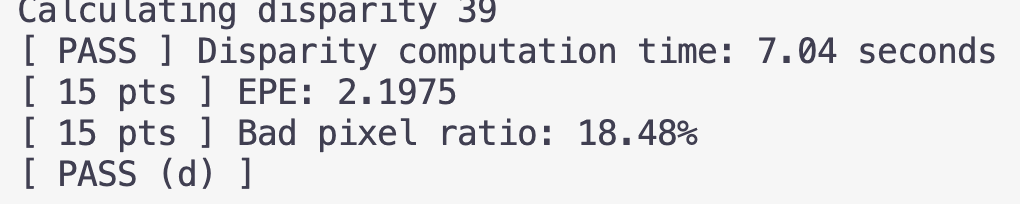
\includegraphics[width=9cm]{../result/result_1.png}
    \caption{Computation Result with window size=30 and disparity range=40}
    \label{fig:result2}
\end{figure}

Choosing the disprity range was quite easy; I first set the max disparity a large value, such as 100. Then I checked out that the most of the disparity are located between 0 to 50. I choosed 40 as max disparity to get rid of the outliers and to calculate bit tightly for large disparities.
\begin{figure}[h]
    \centering
    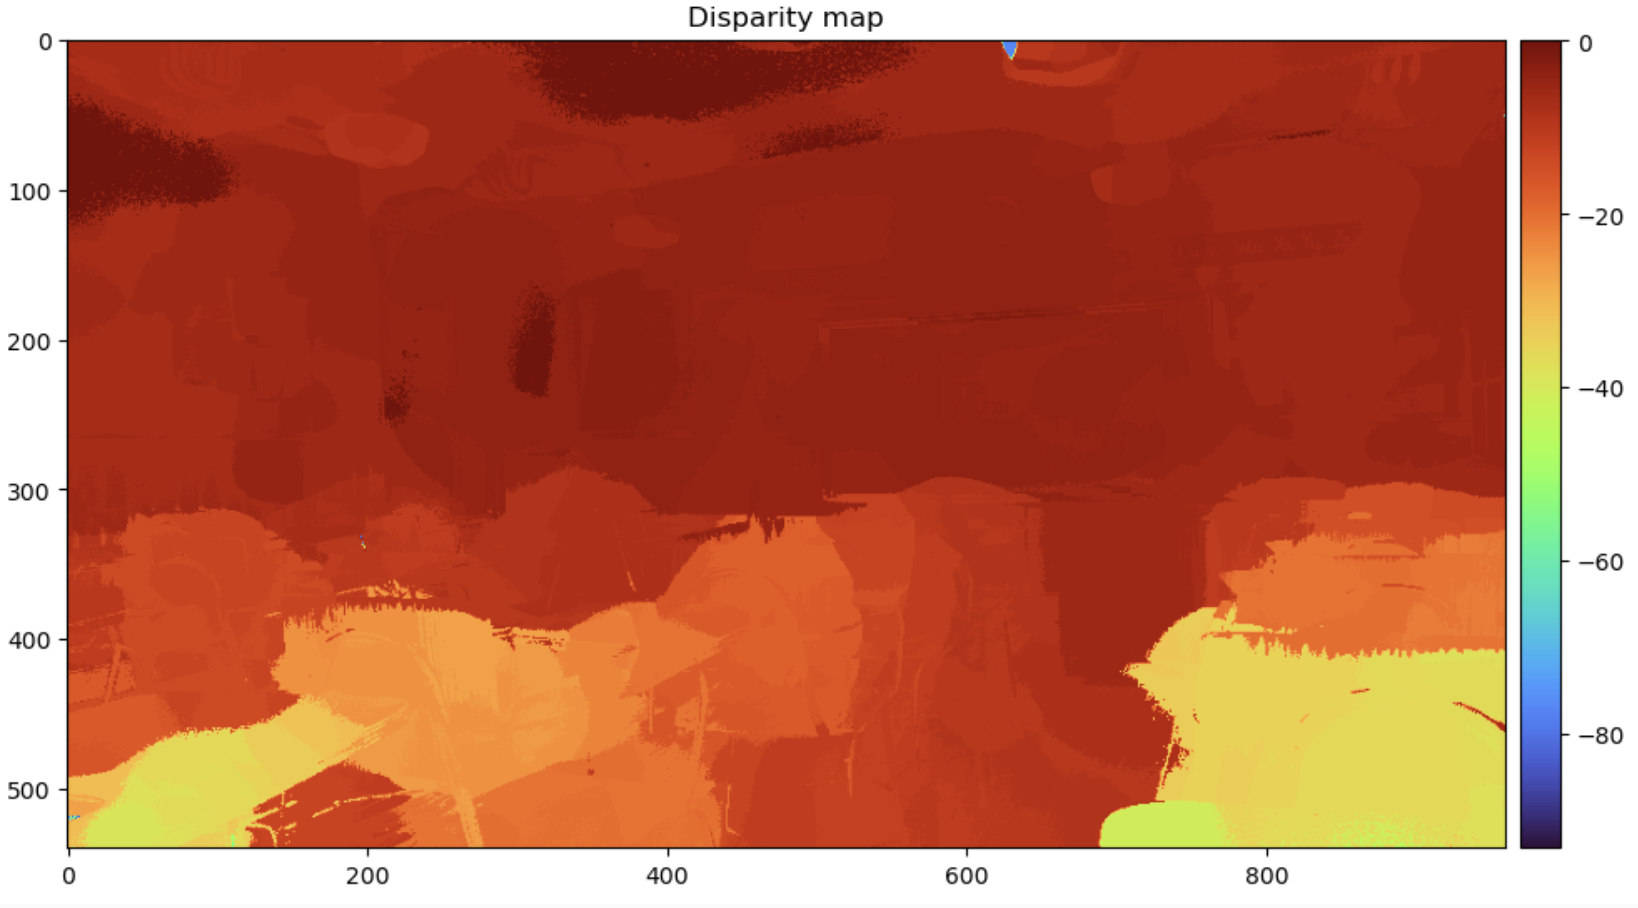
\includegraphics[width=9cm]{../result/disparityragne100.png}
    \caption{Disparity map with max disparity 100. We could notice that most of disparity is smaller than 50.}
    \label{fig:result3}
\end{figure}

Choosing window size was bit confusing. At the beginning I thought the small value will give better result, but oppositely, large size of window made better result. 


\begin{table}[h]
    \centering
    \begin{tabular}{lrrr}
        \toprule
        {Window Size}&{Bad Pixel Ratio (percent)}&{Computation Time{seconds}} \\
        \midrule
        10 & 22.74 & 4.75\\
        20 & 19.67 & 5.64\\
        30 & 18.48 & 6.87\\
        40 & 18.32 & 7.60\\
        50 & 18.56 & 8.68\\
        \bottomrule
    \end{tabular}
    \caption{Window Size vs Bad Pixel Ratio, all other conditions identical.}
    \label{tab:table1}
\end{table}

As noticed in \ref{tab:table1}, the bad pixel ratio start to increase again around 50. I choosed 30 for window size, because bit larger value would give better error ratio but worse in compuational time.

Next, I choosed the parameters for the guided filter, $radius$ and $epsilon$. For $radius$, I used 40, and for epsilon I used $0.1$. Actually the change in this parameter affected the result a lot than I expected, so i just choosed the value empirically. What I noticed that in this project, more smoothing usually leads to better error ratio. Since larger radius and smaller epsilon leads to more smoothing and less edge preservation, it produced better result in error ratio. I think this would vary with different ground truth disparity maps.

\section*{Sub-Pixel Disparity}
I additionally implemented the Sub-Pixel Disparity.
\begin{lstlisting}[language=python]
#Sub-Pixel Disparity
limit = 1e-5  # Smoothing term to prevent division by zero
max_subpixel_correction = 0.5

for y in range(h):
    for x in range(w):
        d = disparity_map[y, x]
        if d == 0 or d == DISPARITY_RANGE - 1:
            continue
        C0 = cost_volume[y, x, d-1]
        C1 = cost_volume[y, x, d]
        C2 = cost_volume[y, x, d+1]

        denominator = 2*(C2 + C0 - 2*C1)
        
        # Check if the denominator is too small or zero
        if np.abs(denominator) < limit:
            continue
        subpixel_correction = (C2 - C0) / denominator
        subpixel_correction = np.clip(subpixel_correction, -max_subpixel_correction, max_subpixel_correction)

        disparity_map[y, x] = d + subpixel_correction
\end{lstlisting}
\begin{enumerate}
    \item \textbf{Limiting the range of Value} 
    $epsilon$ and $max\_subpixel\_correction$ is both the parameter to limit the range of value for subpixel. This will be explained later.
    \item \textbf{Parabolic Fitting} I applied parabolic fitting for each coordinates and three disparities in a row, with regards to this equation:
    \[
d_{\text{sub-pixel}} = d + \frac{C(d-1) - C(d+1)}{2(C(d-1) - 2C(d) + C(d+1))}
\]
which is a parabolic fitting crossing three points.

Since the denominator value could go to zero, I excluded the pixels with denominator value with smaller than limit. 
    \item\textbf{Max Correction} Even after I applied limit, some of the denominator values were too small, making those sub-pixel disparity very large. Thus, I set the max correction value and applied $np.clip()$ to limit the value of correction.

\end{enumerate}
After applying Sub-Pixel Disparity, the bad pixel ratio \textbf{decreased about 0.08 percent}. Though my implementation is not perfect, with a better correction It would give a better result with correction. The disparity map before and after applying sub-pixel disparity is shown in \ref{fig:result4}.
\begin{figure}[h]
    \centering
    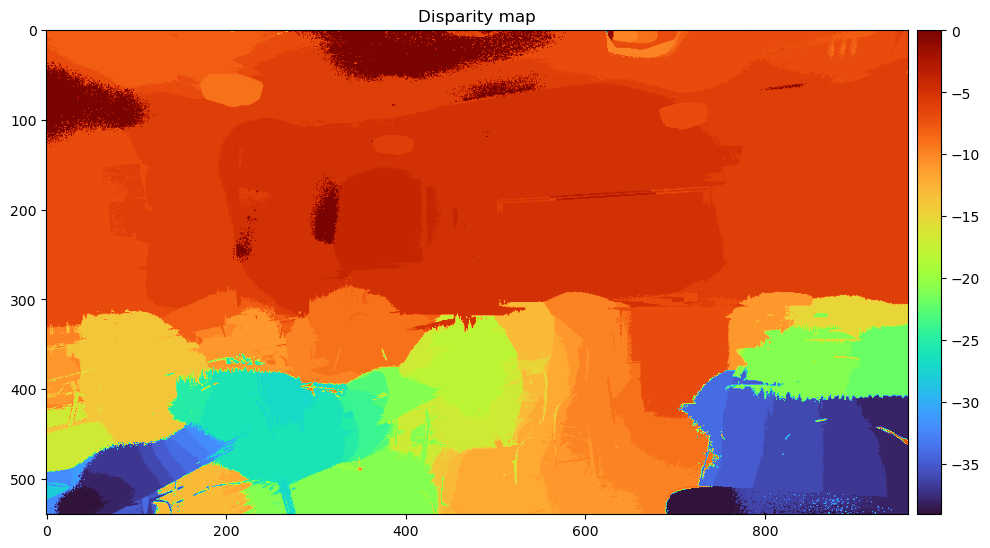
\includegraphics[width=7cm]{../result/disparity_map_nocorrection.png}
    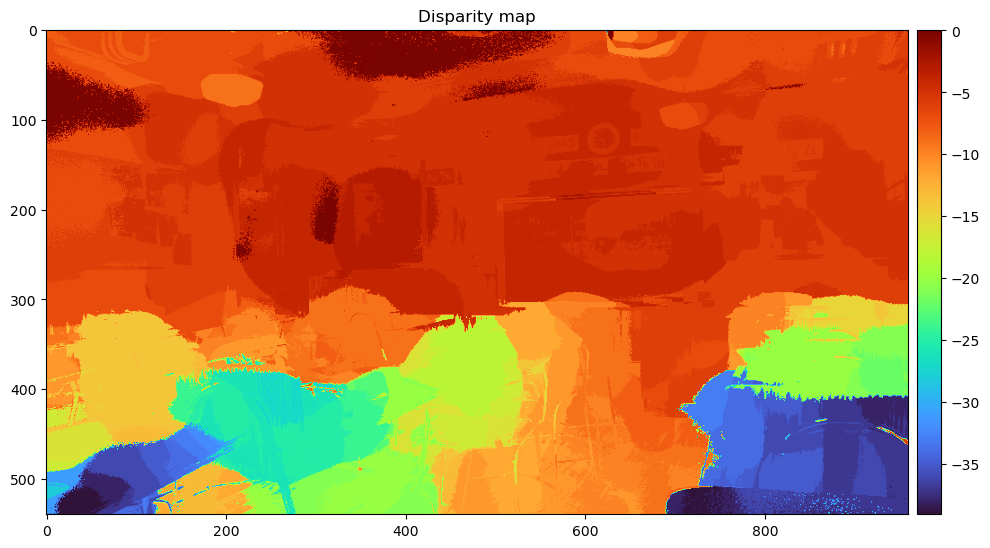
\includegraphics[width=7cm]{../result/disparity_map_correction.png}
    \caption{Top: Withoud Sub-Pixel, Bottom: With Sub-Pixel.}
    \label{fig:result4}
    
\end{figure}
\section*{Box Filter Cost Aggregation}
The original implementation with box filter is this.
\begin{lstlisting}[language=python]
# Box Filter
for d in range(DISPARITY_RANGE):
    cost_volume[:,:,d] = cv2.boxFilter(cost_volume[:,:,d], ddepth=-1, ksize=(30, 30))
\end{lstlisting}
The error seem decreased in big size filters, so I used filter size of 30.
\begin{figure}
    \centering
    \includegraphics*[width=7cm]{../result/disparity_map_box.png}
    \caption{Disparity Map Calculated with Box Filter}
\end{figure}
\section*{Machine Information}
All the results were calculated in M2 Pro Macbook, with 16GB RAM.
\end{document}